\documentclass[12pt, oneside]{article}   	% use "amsart" instead of "article" for AMSLaTeX format
\usepackage{textcomp}
\usepackage{geometry}                		% See geometry.pdf to learn the layout options. There are lots.
\geometry{letterpaper}                   		% ... or a4paper or a5paper or ... 
%\geometry{landscape}                		% Activate for rotated page geometry
%\usepackage[parfill]{parskip}    		% Activate to begin paragraphs with an empty line rather than an indent
\usepackage{graphicx}				% Use pdf, png, jpg, or eps§ with pdflatex; use eps in DVI mode
\usepackage{caption}
\usepackage{subcaption}								% TeX will automatically convert eps --> pdf in pdflatex		
\usepackage{color}
\usepackage{amssymb}
\usepackage{amsthm}
\usepackage{url}
\newtheorem{theorem}{Theorem}
\newtheorem{definition}{Definition}
\usepackage{natbib}
\usepackage{xcolor}
% removed hyperref because of arXiv complaining
\usepackage{authblk}
\usepackage{float}
\usepackage{rotating}
\usepackage{adjustbox}
\usepackage[font=small,labelfont=bf]{caption}
%\usepackage{changes}
\usepackage{changes}
\definechangesauthor[name={George Chacko}, color=blue]{gc}

\usepackage{authblk}
\title{Finding Well-Connected Communities in Real-World Networks}
\author[1]{Minhyuk Park\thanks{author order to be determined later}}
\author[1]{Yasamin Tabatabaee\thanks{author order to be determined later}}
\author[1]{Baqiao Liu\thanks{author order to be determined later}}
\author[1]{Placeholder1\thanks{author order to be determined later}}
\author[1]{Placeholder2\thanks{author order to be determined later}}
\author[1]{Placeholder3\thanks{author order to be determined later}}
\author[2]{Dmitriy Korobskiy}
\author[1,3]{George Chacko\thanks{warnow@illinois.edu}}
\author[1]{Tandy Warnow\thanks{chackoge@illinois.edu}}
\affil[1]{Department of Computer Science, University of Illinois Urbana-Champaign, Urbana, IL 61801}
\affil[2]{NTT DATA, McLean, VA 22102}
\affil[3]{Office of Research, Grainger College of Engineering, University of Illinois Urbana-Champaign, Urbana, IL 61801}

% \setlength{\parindent}{0pt}
%SetFonts

% ORCID IDs

% Baqiao Liu: 0000-0002-4210-8269
% Tandy Warnow: 0000-0001-7717-3514
% George Chacko: 0000-0002-2127-1892

\begin{document}
\maketitle
	
\abstract{Community detection in real-world networks is a basic step in scientometrics research, and is typically addressed through the use of
graph clustering methods that partition the vertices of a network into disjoint subsets.
While  the formal definition for ``community" vary across methods, it is well accepted that a community should be well-connected, so that the deletion of a small
number of edges should not disconnect the community.
Here, we evaluate how well-connected the clusters are that are produced using two 
 approaches for graph clustering -- the Leiden software using different resolution parameters
and Iterative k-core clustering (Wedell et al., QSS 2022). 
We find that both methods produce clusters that are poorly connected when applied to real-world networks, but this is especially true for Leiden when run
with small resolution parameter values.
We present a new pipeline for use with these clustering methods that guarantees that the output clusters will be well-connected, and explore its use
on a collection of real world networks, including several citation networks, and their  corresponding synthetic LFR networks.
Used with Leiden and IKC, our study suggests that only a fraction (ranging from x\% to 80\%) of  the  vertices in real world networks are found in 
well-connected communities containing at least 11 vertices.
Interestingly, when applied to the corresponding synthetic LFR networks, a different pattern is observed: most of the network is 
contained in well-connected clusters containing at least 11 vertices.
Since the LFR network generation process by definition assumes that every vertex is in a community, this 
study suggests the possibility that community structure is not globally found within real-world networks, and that clusters produced by
standard methods should be post-processed to evaluate whether they satisfy criteria for being a valid community.
The pipeline we provide is tunable to allow the user to specify the criteria for a valid community in terms of (a)  a lower bound on the community size and (b) the 
minimum edge cut size as a function of the cluster size. 
}
	
\clearpage
	
\section{Introduction} 

The problem of finding communities in complex networks can be posed as a {\em graph partitioning} problem, where the input is a network (a graph with vertices and edges) and the
objective is a partitioning of the vertices into disjoint subsets, so that each of the subsets represents a community. While variants of this formulation exist \citep{Coscia2011}, constructing 
overlapping clusters for example, this is a common approach to community detection that has been used in many studies \citep{Fortunato2022,Fortunato2010}. Community detection in 
large networks has broad applications that include, in scientometrics, the detection of research areas, and author communities [cite Waltman].

While definitions of what constitutes a community vary, a common assumption is that elements of community are more connected to each other than to those outside the community. 
In other words, that a community will be {\em well-connected}. Well connected can be further clarified by asserting that for a cluster to define a valid community, it  should not have a small 
edge cut, i.e., there should not be a small set of edges whose deletion disconnects the cluster; see discussion in \citep{Traag_2019}. 


While the minimum size of an edge cut is a matter that can be debated, two formulations have been proposed for this.
The first approach simply requires that an edge cut be above some size that depends on the number $n$ of vertices in the cluster, such as $\log_{10}(n)$. 
This is a relatively weak bound for large values of $n$, but does provide some constraints on small clusters (e.g., a tree cluster with ten or more vertices would be considered to be poorly connected).  
The second approach, which is used in providing guarantees for the Leiden clustering, evaluates the size of an edge cut by the split  of the cluster into two parts produces when the edge cut is removed from a cluster, and requires that the
edge cut size be at least a fraction of the number of possible edges between the two  parts.
As proven in \citep{Traag_2019} (Equation D1 in the supplementary information), 
given any optimal CPM clustering of a network using resolution parameter $\gamma$, if an edge cut $E_0$
separates a cluster into two sets $A$ and $B$, then the edge cut has at least $\gamma ||A|| \times ||B||$, where
$||.||$ indicates the number of vertices in the given set.
This is a strong guarantee for large clusters,  but as it depends on the value for $\gamma$, it may have no guarantee  beyond being connected for small clusters
(see Discussion). 
% (below, for example,  $2\sqrt \frac{1}{\gamma}$).

Given the importance of communities being well-connected, we performed a study to evaluate the question of whether clusters produced by different clustering methods
were consistently found to be well-connected, using the first criterion we pose, so that for every cluster, the minimum edge-cut size must be greater than $\log_{10}n$, where $n$ is the number of vertices in the cluster. 
We used a collection of real-world networks in our study, including some citation graphs (e.g., the Curated Exosome Network \citep{Wedell2022})  but also including networks of other types from the Stanford Network Analysis Platform (SNAP) \citep{leskovec2016snap}.
This evaluation showed that both Leiden and IKC clusterings produced clusters that failed to be well-connected according to this criterion.
The results depended on the resolution parameter selected for Leiden,  with a higher incidence of failure for small values for the resolution parameter.

We then designed a pipeline to work with both Leiden and IKC that would ensure that all output clusters satisfy two constraints for being valid communities: (1) they are well-connected, according to our criterion, and (2) each cluster is not too small (by default, we require that each cluster have at least 11 vertices).
The pipeline takes the clustering as input, and first finds and removes all clusters that are either trees or are too small.  It then checks each remaining cluster for being well-connected; if a cluster
fails this check so that it has a small edge cut, the minimum edge cut is deleted from the cluster, thus producing a set of subsets.  Each of these subsets are then re-clustered using the selected clustering
method (IKC or Leiden), and the process recurses on the resultant set of clusters.

Our study using this pipeline on a collection of real-world networks shows some surprising results.
First, we find that the final clustering produced using Leiden, across a range of resolution values, 
covered only a portion of the input network, with a  fraction that ranged from x\% to y\% of the vertices.

\textcolor{blue}{TO do:
\begin{itemize}
\item Report the fraction of input clusters that fail our test as a function of the cluster size.
We expect this to be a large fraction for small clusters but it may continue into the larger clusters.
Will be good to note.
\item Look at how much of the network is in the *union* of the output (post-pipeline) clusterings, across the Leiden resolution parameter values.
\item Compute the overlap between clusterings both pre-pipeline and post-pipeline
\item  Evaluate accuracy of Leiden clusterings on LFR networks 
\end{itemize}
}

\section{Materials and Methods}

\subsection{Methods} 
\emph{Pipeline} A modular pipeline was developed that (i) generated a clustering from an input network (ii) filtered the resultant clusters to remove small clusters ($<$ 10 nodes) and trees (the case where the sum of internal edges in a cluster was one less than the number of nodes in the same cluster) (iii) applied \emph{Connectivity Modifier} (CM), a recursive minimum cut to each filtered cluster to ensure well-connectedness.

\vspace{5 mm}
\textbf{[Insert flow chart of workflow/pipeline]}

\subsubsection{Clustering} insert text
\subsubsection{Filters} insert text
\subsubsection{Connectivity Modifier} insert text 

\subsection{Data} Several networks were used for testing and analysis and were selected to provide a range of sizes and edge density. In all cases, below the counts of nodes and edges are reported after removing duplicate records, 
self-citations, and parallel edges from the source data. \emph{Curated Exosome Network (CEN)}. The CEN is centered around the exosome research literature. Its construction has previously been previously described in \citep{Jakatdar_2022}, and it consists of 13,989,436 nodes and 92,051,051 edges.  \emph{Open Citations} A custom-implemented ETL process was designed to process the publicly available OpenCitations dataset \citep{Peroni2020} and load it into a PostgreSQL table. Citation data (CSV) was downloaded in Aug 2022. A custom ETL script, written in Bash and SQL, was used to find and pipe uncompressed CSV files, in 20 parallel jobs using the GNU Parallel command-line utility, to a custom function which loaded individual CSV files into a staging view. DOIs were also checked for case differences to remove duplicates.  The resultant network contained 75,025,194 nodes and 1,363,605,603 edges.  In addition, four more real world networks from the Stanford Network Analysis Project (SNAP) collection \citep{leskovec2016snap} were downloaded in Dec 2022: \emph{cit\_patents} (3,774,768 nodes, 16,518,947 edges), \emph{cit\_hepph} (34,546 nodes, 420,877 edges), \emph{wiki\_topcats} (1,791,489 nodes, 25,444,207 edges), and \emph{orkut} (3,072,441 nodes, 117,185,083 edges). As a comparison group, synthetic networks were generated using the LFR `benchmark' methodology \citep{Lancichinetti2008}. [Ask Yasamin to write this section up].

\section{Results and Discussion}

\emph{Overview editorial for consideration by authors. We need to agree on a vision to integrate the Leiden and IKC results into an overarching hypothesis-driven framework. What is it that we're looking for. To me, the answer is in an improved understanding of how the the properties of networks affect clustering and the converse- how clustering methods influence interpretation of the networks that are fed to them. Are we asking too much of ourselves? Should the IKC effort be in its own paper? My sense is that IKC is a valuable comparison method because of the way in which it is so different from Leiden and perhaps less valuable because it's so different from Leiden.}

\textcolor{blue}{\emph{Assuming that we want to have `our very best figure' early, if not first, what should it be?}} I think it should be the CEN tree figure, which would justify exploring other networks.  Does this distract from the focus on connectivity modifier?

\begin{figure}[H]
\centering
\includegraphics[width=0.7\linewidth]{discussion_1.pdf}
\caption{For the purpose of discussion, the clustering of the CEN with Leiden-CPM at res 0.01 results in around 85\% node coverage considering clusters of size $>$ 10. The network consists of roughly 13.9 million nodes. The number of such clusters is 65,771 AND 35\% of them are trees (green). I set alpha to 0.05 to indicate overplotting effects else 35\% would seem unlikely. The order and motivation of our exposition could therefore be...``In an extended examination of the features of clusters in a network we have previously studied, we observed that a significant fraction were trees, which are the minimally dense state of a connected cluster. This motivated us to empirically examine the output of the Leiden algorithm with its guarantees of well connected clusters and ask whether features of the network affected such guarantees.'' Thus, the CEN would be our Eureka observation but it should be made clear that the hypothesis follows the serendipitous finding.}
\end{figure}

	
\begin{figure}[H]
\centering
\begin{subfigure}[t]{0.48\textwidth}
\centering
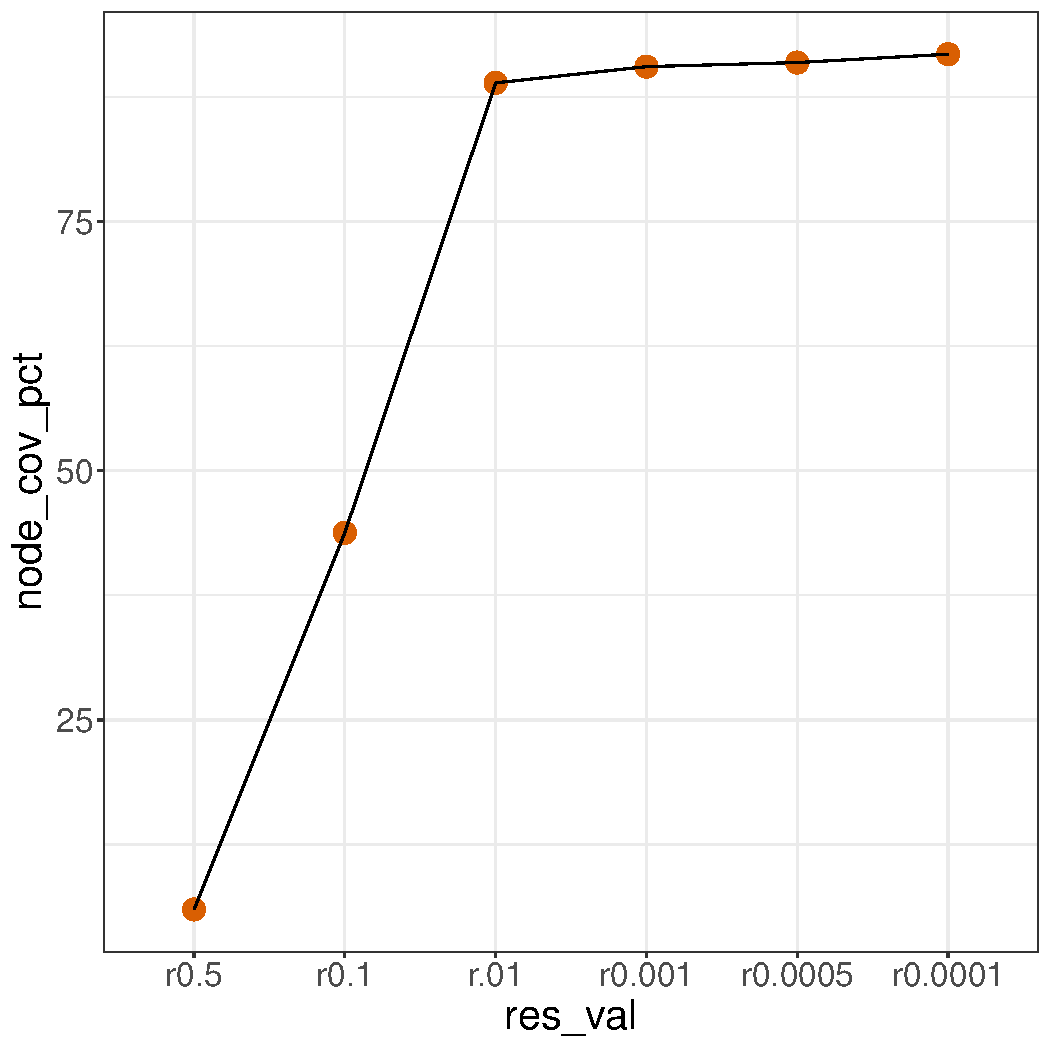
\includegraphics[width=\linewidth]{node_cov.pdf}
\end{subfigure}
\hfill
\begin{subfigure}[t]{0.48\textwidth}
\centering
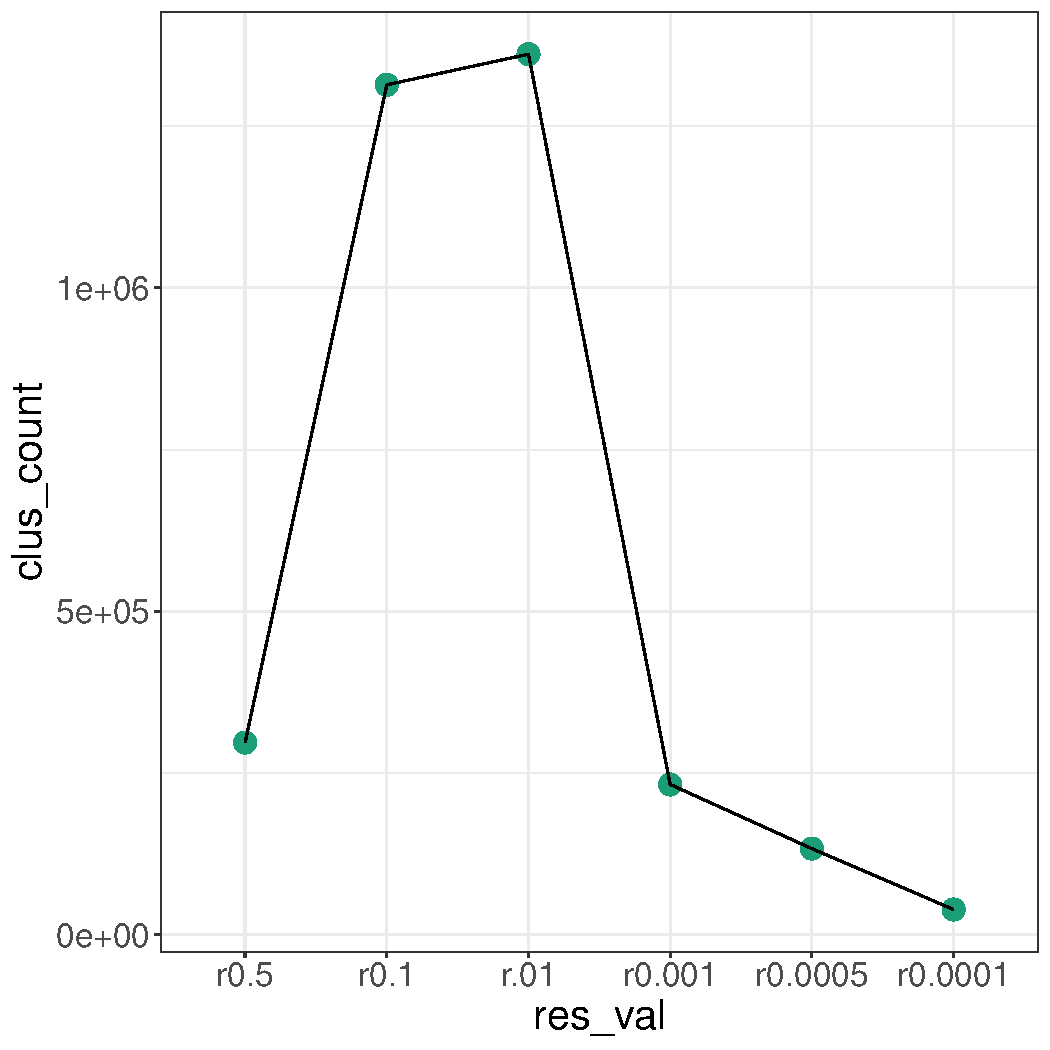
\includegraphics[width=\linewidth]{clus_count.pdf} 
\end{subfigure}
\captionsetup{width=0.9\textwidth}
\caption{Draft Comments: As res\_val decreases, node coverage increases although the number of N$>$10 clusters first goes up then falls. Thus cluster size must be increasing. See Table 1}
\label{fig:overlapping}
\end{figure}



% latex table generated in R 4.2.2 by xtable 1.8-4 package
% Fri Jan 13 18:03:02 2023
\begin{table}[ht]
\centering
\begin{tabular}{rrrrrr}
  \hline
 res\_value & clus\_count & node\_cov & min & med & max \\ 
  \hline
0.5 & 297038 & 5.98 &  11 & 13.00 & 183 \\ 
0.1 & 1313856 & 43.78 &  11 & 17.00 & 882 \\ 
0.01 & 1361168 & 88.93 &  11 & 19.00 & 3530 \\ 
0.01 & 232288 & 90.56 &  11 & 64.00 & 23470 \\ 
0.0005 & 133147 & 90.97 &  11 & 90.00 & 39049 \\  
0.0001 & 39069 & 91.81 &  11 & 177.00 & 176557 \\ 
   \hline
\end{tabular}
\caption{Clustering the Open Citations Network. The open citations network (Materials and Methods) consisting of 75,025,194 nodes and 1,363,605,603 edges was clustered with the Leiden algorithm, using the Constant Potts Model (CPM ) as quality function, and using various resolution values (column 1). Node coverage is expressed as the the percent of nodes in these clusters of size $>$ 10 relative to the total number of nodes in the network. Minimum, median, and max cluster sizes are shown in the last three columns.  }
\end{table}


		
\section{Conclusions}
	
\section*{Competing Interests} \vspace{3mm} The authors have no competing interests. 
	
\section*{Funding Information} 
	
\section*{Data Availability} 
	
\section*{Acknowledgments} 

\bibliographystyle{apalike}
\bibliography{cmv1}
\end{document}


